\documentclass[conference,a4paper]{IEEEtran}

\usepackage[T1]{fontenc}
\usepackage[spanish]{babel}

\usepackage{amsmath}
\usepackage{graphicx}
\usepackage[kw]{pseudo}
\usepackage{booktabs}
\usepackage{cite}
\usepackage{hyperref}
\usepackage{float}
\usepackage{titlesec}

\titlespacing*{\section}{2pt}{2pt}{1pt}
\titlespacing*{\subsection}{2pt}{2pt}{1pt}

\def\contentsname{Índice general}
\def\listfigurename{Índice de figuras}
\def\listtablename{Índice de tablas}
\def\refname{Referencias}
\def\indexname{Índice alfabético}
\def\figurename{Fig.}
\def\pseudoname{Pseudocódigo}
\def\tablename{TABLA}
\def\partname{Parte}
\def\appendixname{Apéndice}
\def\abstractname{Resumen}
\def\IEEEkeywordsname{Palabras clave}
\def\IEEEproofname{Demostración}

\begin{document}

\title{Desarrollo de un Agente Inteligente para Otelo basado en MCTS-UCT y Redes Neuronales} 

\author{
  \IEEEauthorblockN{Nuno José del Pino Escalante} 
  \IEEEauthorblockA{
    \textit{Dpto. Ciencias de la Computación e Inteligencia Artificial}\\ 
    \textit{Universidad de Sevilla}\\ 
    Sevilla, España\\ 
    nundelesc@alum.us.es} 
  
  \and
  
  \IEEEauthorblockN{Javier Gutiérrez Pastor} 
  \IEEEauthorblockA{
    \textit{Dpto. Ciencias de la Computación e Inteligencia Artificial}\\ 
    \textit{Universidad de Sevilla}\\ 
    Sevilla, España\\ 
    javgutpas@alum.us.es} 
}

\maketitle

\begin{abstract}
  Este trabajo tiene como objetivo el desarrollo de un agente capaz de jugar a Otelo utilizando una combinación de técnicas de búsqueda y aprendizaje profundo. 
Como base del agente se emplea el algoritmo Monte Carlo Tree Search (MCTS) utilizando el enfoque Upper Confidence Bounds for Trees (UCT), encargado de explorar las posibles jugadas y seleccionar aquellas que parecen más prometedoras. 

Con el objetivo de mejorar la toma de decisiones, se entrena una red neuronal a partir de partidas generadas automáticamente por el propio agente. 
Una vez entrenada, esta red se utiliza para evaluar estados del tablero durante la búsqueda, sustituyendo las simulaciones aleatorias empleadas inicialmente. 

Por último, se realizan diferentes experimentos para analizar tanto la calidad de las predicciones de la red neuronal como el rendimiento general del agente. 
Los resultados obtenidos permiten estudiar las ventajas y limitaciones de combinar UCT y aprendizaje profundo en el juego de Otelo. 
\end{abstract}

\begin{IEEEkeywords}
  Otelo, MCTS, UCT, Red Neuronal, Agente, Modelo, Inteligencia Artificial. 
\end{IEEEkeywords}

\section{Introducción} 

Otelo, también conocido como Reversi, es un juego de estrategia para dos jugadores que se desarrolla sobre un tablero de 8x8 casillas. 
El objetivo consiste en tener la mayoría de las fichas de tu color sobre el tablero al finalizar la partida. 
Solo se pueden colocar fichas en casillas vacías de manera que, en línea recta (horizontal, vertical o diagonal) una o más fichas del oponente queden atrapadas, haciendo así que éstas pasen a ser del color del jugador que hizo la jugada. 
Si ninguno de los jugadores puede realizar un movimiento válido o si todas las casillas del tablero están ocupadas, la partida finaliza. 
Aunque sus reglas son relativamente sencillas, la gran cantidad de posiciones posibles y la necesidad de planificar movimientos a largo plazo hacen que resulte un entorno muy interesante para aplicar técnicas de inteligencia artificial. 

En los últimos años, los juegos de tablero como go, shogi o ajedrez han servido como banco de pruebas para numerosos algoritmos de toma de decisiones. 
Entre ellos destacan los métodos de búsqueda adversaria y, más recientemente, los enfoques que combinan búsqueda y aprendizaje profundo. 
Sistemas como "AlphaGo"~\cite{b1} o "AlphaZero"~\cite{b2} demuestran que la utilización conjunta de estas técnicas puede dar lugar a agentes capaces de alcanzar un nivel de juego muy alto. 

Siguiendo esta idea, el objetivo principal de este trabajo es desarrollar un agente para Otelo basado en Monte Carlo Tree Search (MCTS), utilizando la estrategia Upper Confidence Bounds for Trees (UCT) para guiar la exploración del árbol de búsqueda. 
En una primera fase, se implementa un agente basado exclusivamente en UCT, que posteriormente se utiliza para generar partidas mediante autojuego. 
Para ello, el agente disputa partidas contra sí mismo, seleccionando movimientos mediante el algoritmo de búsqueda implementado. 

A partir de estas partidas se construye un conjunto de datos de entrenamiento formado por estados del tablero y sus correspondientes resultados finales obtenidos. 
Con esta información se entrena una red neuronal capaz de estimar la calidad de una posición de juego. 
Una vez entrenada, la red se integra en el agente con el objetivo de mejorar la evaluación de los estados explorados durante la búsqueda. 

Además del desarrollo del agente, este trabajo pretende analizar hasta qué punto la incorporación de la red neuronal puede reemplazar las simulaciones aleatorias utilizadas por UCT, proporcionando evaluaciones más precisas y favoreciendo la toma de decisiones del agente. 
Para ello, se comparan distintas configuraciones del agente y se estudia tanto la calidad de las predicciones realizadas por la red como el comportamiento observado durante las partidas. 

Este documento se organiza en seis secciones, incluyendo la presente introducción. 
En la Sección II se describen en mayor detalle las técnicas empleadas y se revisan algunos trabajos relacionados. 
En la Sección III se expone la metodología seguida y se detalla la implementación del sistema. 
La Sección IV está dedicada a los experimentos realizados y al análisis de los resultados obtenidos. 
En la Sección V se presentan las conclusiones del proyecto, así como posibles líneas futuras de mejora. 
Finalmente, la sección VI incluye la declaración de uso de inteligencia artificial generativa. 
Las referencias bibliográficas utilizadas se presentan al final del documento. 

\section{Preliminares} 

\subsection{Monte Carlo Tree Search} 
Monte Carlo Tree Search (MCTS) es un algoritmo de búsqueda ampliamente utilizado para la toma de decisiones en problemas donde el espacio de estados es muy grande. 
Su funcionamiento se basa en la construcción progresiva de un árbol de búsqueda mediante la realización de múltiples simulaciones a partir del estado de juego actual. 

Cada iteración de MCTS se compone de cuatro fases principales: 
\begin{itemize}
\item Selección: Se recorre el árbol desde la raíz siguiendo la política de selección hasta alcanzar un nodo hoja o un nodo no completamente expandido. 
\item Expansión: Se añaden nuevos nodos correspondientes a movimientos aún no explorados. 
\item Simulación: Se estima el resultado de la partida a partir del estado alcanzado, es decir se juega una partida simulada desde el nuevo nodo hasta alcanzar un estado terminal. 
\item Retropropagación: El resultado obtenido en la simulación se propaga hacia atrás actualizando las estadísticas de los nodos visitados. 
\end{itemize}

A medida que aumenta el número de simulaciones, el algoritmo dispone de más información para estimar la calidad de cada movimiento y seleccionar las acciones más prometedoras. 
El proceso se repite hasta agotar el presupuesto computacional disponible. 
Finalmente, el agente selecciona la acción asociada al nodo que ha mostrado mejor comportamiento durante la búsqueda. 

El Pseudocódigo 1 muestra el funcionamiento general de la variante UCT empleada en este trabajo. 

\newpage

\begin{figure}[t]
  \noindent
  \begin{minipage}{\columnwidth}
    \begin{pseudo}[compact, left-margin=0pt, label-align=l]
      \textbf{Función UCTSEARCH}($s_0$) \\ 
      \> Crear nodo raíz $v_0$ con estado $s_0$ \\ 
      \> \textbf{Mientras} esté dentro del presupuesto computacional \\ 
      \> \> $v_i \leftarrow \text{TREEPOLICY}(v_0)$ \\ 
      \> \> $\Delta \leftarrow \text{DEFAULTPOLICY}(s(v_i))$ \\ 
      \> \> \text{BACKUP}$(v_i, \Delta)$ \\ 
      \> \textbf{Devolver} $a(\text{BESTCHILD}(v_0, 0))$ \\ 

      \\

      \textbf{Función TREEPOLICY}($v$) \\ 
      \> \textbf{Mientras} $v$ es no terminal \\ 
      \> \> \textbf{Si} $v$ no está totalmente expandido \\ 
      \> \> \> \textbf{Devolver} \text{EXPAND}($v$) \\ 
      \> \> \textbf{Sino} \\ 
      \> \> \> $v \leftarrow \text{BESTCHILD}(v, C_p)$ \\ 
      \> \textbf{Devolver} $v$ \\ 

      \\

      \textbf{Función EXPAND}($v$) \\ 
      \> Escoger $a \in$ acciones sin intentar de $A(s(v))$ \\ 
      \> Añadir nuevo hijo $v'$ a $v$ \\ 
      \> \> Con $s(v') = f(s(v), a)$ \\ 
      \> \> Y $a(v') = a$ \\ 
      \> \textbf{Devolver} $v'$ \\ 

      \\

      \textbf{Función BESTCHILD}($v, c$) \\ 
      \> \textbf{Devolver} \mbox{$\displaystyle \arg\max_{v' \in \text{hijos de } v} \left( \frac{Q(v')}{N(v')} + c \sqrt{\frac{2 \ln N(v)}{N(v')}} \right)$} \\ 

      \\

      \textbf{Función DEFAULTPOLICY}($s$) \\ 
      \> \textbf{Mientras} $s$ no es terminal \\ 
      \> \> Escoger $a \in A(s)$ de manera \\ 
      \> \> uniformemente aleatoria \\ 
      \> \> $s \leftarrow f(s,a)$ \\ 
      \> \textbf{Devolver} recompensa para el estado $s$ \\ 

      \\

      \textbf{Función BACKUP}($v, \Delta$) \\ 
      \> \textbf{Mientras} $v$ es no nulo \\ 
      \> \> $N(v) \leftarrow N(v) + 1$ \\ 
      \> \> $Q(v) \leftarrow Q(v) + \Delta$ \\ 
      \> \> $\Delta \leftarrow -\Delta$ \\ 
      \> \> $v \leftarrow$ padre de $v$ 
    \end{pseudo}
  \end{minipage}
  \vspace{0.5em}
  \label{pcd:uct}
\end{figure}

\subsection{Upper Confidence Bounds for Trees} 
Upper Confidence Bounds for Trees (UCT) es una variante de Monte Carlo Tree Search que emplea la estrategia Upper Confidence Bound (UCB) para decidir qué nodos explorar durante la fase de selección. 
Su objetivo es equilibrar dos aspectos fundamentales del proceso de búsqueda: la exploración de movimientos poco visitados y la explotación de aquellos que han mostrado buenos resultados en simulaciones anteriores. 

Para ello, a cada nodo del árbol se le asigna un valor calculado mediante la ecuación (1): 

\begin{equation}
UCT(v)=\frac{Q(v)}{N(v)}+C*\sqrt{\frac{ln(N(p))}{N(v)}} 
\end{equation}

donde: 
\begin{itemize}
\item $Q(v)$ representa la recompensa acumulada obtenida por el nodo (v). 
\item $N(v)$ indica el número de veces que el nodo ha sido visitado. 
\item $N(p)$ corresponde al número de visitas realizadas al nodo padre. 
\item $C$ es una constante que controla el equilibrio entre exploración y explotación. 
\end{itemize}

En este trabajo se ha utilizado el valor $C=\frac{1}{\sqrt{2}}$, por lo que la expresión empleada durante la búsqueda queda representada por la ecuación (2): 
\begin{equation}
UCT(v) = \frac{Q(v)}{N(v)} + \frac{1}{\sqrt{2}}\sqrt{\frac{ln(N(p))}{N(v)}} 
\end{equation}

Gracias a este criterio, el algoritmo favorece la exploración de movimientos que han sido analizados pocas veces, sin dejar de priorizar aquellos que han obtenido buenos resultados. 
De esta manera, UCT consigue dirigir la búsqueda hacia las regiones más prometedoras del árbol, mejorando progresivamente la calidad de las decisiones tomadas por el agente. 

\subsection{Redes neuronales multicapas} 
Las redes neuronales multicapas son modelos de aprendizaje capaces de aproximar funciones complejas a partir de ejemplos de entrenamiento. 
Durante el proceso de aprendizaje, la red ajusta sus parámetros internos para establecer relaciones entre las entradas recibidas y los valores objetivo asociados~\cite{b4}. 

En este trabajo se emplea una arquitectura convolucional de tipo feedforward, compuesta por varias capas ocultas. 
El entrenamiento se realiza mediante aprendizaje supervisado, utilizando ejemplos para los que se conoce previamente la salida~\cite{b3}. 
De esta forma, las predicciones generadas por la red pueden compararse con los valores reales, permitiendo ajustar progresivamente sus parámetros para mejorar su precisión. 

Para ello, la red recibe como entrada una representación del estado de la partida y produce como salida una valoración numérica de la calidad de la posición correspondiente. 
Una vez entrenada, esta valoración puede utilizarse para guiar el proceso de búsqueda y proporcionar estimaciones más informadas que las obtenidas mediante simulaciones completamente aleatorias. 

\subsection{Aprendizaje mediante autojuego} 
El autojuego es una técnica ampliamente utilizada en la inteligencia artificial para generar datos de entrenamiento sin necesidad de disponer de partidas etiquetadas manualmente. 
Consiste en enfrentar un agente contra sí mismo y registrar la información obtenida durante las partidas. 

En el contexto de este proyecto, el agente basado en UCT juega múltiples partidas contra una copia de sí mismo. 
Durante cada partida se almacenan los estados visitados y, una vez finalizada, se asocia a cada estado el resultado obtenido por el jugador correspondiente. 
Este procedimiento permite generar automáticamente un conjunto de datos que posteriormente se emplea para entrenar la red neuronal encargada de evaluar los estados del tablero. 

\subsection{Trabajo relacionado} 

Una de las principales referencias utilizadas durante el desarrollo de este trabajo ha sido el artículo "A Survey of Monte Carlo Tree Search Methods"~\cite{b5}. 
Este trabajo proporciona una visión detallada de los algoritmos MCTS y, en particular, de la variante UCT, permitiendo comprender sus fundamentos teóricos y su aplicación en problemas de toma de decisiones. 
Además, tanto las explicaciones como el pseudocódigo presentado en dicho artículo sirvieron como guía para la implementación del agente desarrollado. 

Por otra parte, la combinación de búsqueda adversaria y aprendizaje profundo ha dado lugar a algunos de los avances más relevantes en inteligencia artificial aplicada a juegos. 
En este ámbito destacan especialmente los trabajos de "AlphaGo"~\cite{b6} y "AlphaZero"~\cite{b7}, que demostraron el potencial de integrar redes neuronales profundas (Deep Learning) con algoritmos de búsqueda para alcanzar niveles de juego extraordinariamente altos en distintos juegos de tablero. 

Finalmente, también se tomó como referencia un proyecto reciente similar a este centrado en el desarrollo de un agente para Otelo~\cite{b8}. 
Aunque dicho trabajo emplea técnicas diferentes, basadas principalmente en el algoritmo minimax y la poda alfa-beta, constituye un ejemplo interesante de las distintas aproximaciones que pueden utilizarse para abordar este juego desde la perspectiva de la inteligencia artificial. 

\section{Metodología e Implementación} 

\subsection{Implementación del juego Otelo} 
Como base para el desarrollo del agente se implementó una versión completa del juego de Otelo en Python. 
Esta implementación se encarga de gestionar todas las reglas del juego y de proporcionar el entorno necesario para ejecutar partidas, tanto durante el proceso de búsqueda como durante la generación de datos de entrenamiento. 

En una primera fase, el sistema permitía disputar partidas mediante una sencilla interfaz de línea de comandos, donde los movimientos eran introducidos manualmente por el usuario. 
Puesto que el agente aún no había sido desarrollado, esta versión inicial sirvió para comprobar el correcto funcionamiento de las reglas del juego, la validación de movimientos y la actualización del tablero tras cada jugada. 
Una vez verificada su correcta operación, esta implementación se utilizó como base para el desarrollo de los agentes y para la simulación automática de partidas. 

El tablero se representa mediante una matriz de $8\times8$ posiciones, donde cada casilla puede encontrarse vacía o contener una ficha de alguno de los dos jugadores. 
A partir de esta representación se implementan las operaciones necesarias para determinar los movimientos legales disponibles en cada turno, aplicar las capturas correspondientes y actualizar el estado del tablero tras cada jugada. 

\begin{figure}[htbp]
  \centering
  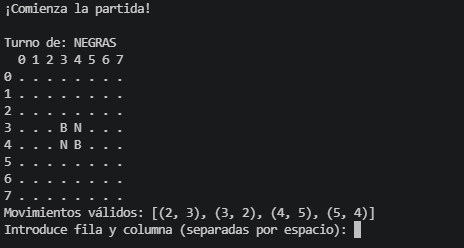
\includegraphics[width=0.8\columnwidth]{interfaz}
  \caption{Fig 1. Interfaz del juego, mostrando el turno del jugador} 
  \label{fig:interfaz}
\end{figure}

Además, el sistema contempla situaciones especiales propias del juego, como la ausencia de movimientos válidos para un jugador, obligándole a ceder el turno al oponente. 
También se implementan los mecanismos necesarios para detectar el final de una partida y determinar el resultado obtenido por cada jugador. 
Esta implementación constituye la base sobre la que se apoyan tanto el algoritmo de búsqueda UCT como el proceso de autojuego que se utiliza posteriormente para generar el conjunto de entrenamiento. 

\subsection{Implementación del agente UCT} 
Una vez implementado el entorno de juego, se desarrolló un agente basado en Monte Carlo Tree Search utilizando la estrategia Upper Confidence Bounds for Trees (UCT) para guiar la exploración del árbol de búsqueda. 

La estructura principal del algoritmo está formada por nodos que almacenan la información necesaria para el proceso de búsqueda, incluyendo el estado del tablero asociado, el jugador al que corresponde el turno, el número de visitas recibidas y la recompensa acumulada obtenida durante las evaluaciones realizadas. 
Asimismo, cada nodo mantiene referencias a su nodo padre y a sus posibles hijos, permitiendo construir y recorrer el árbol de forma eficiente. 

Durante cada iteración del algoritmo se ejecutan las cuatro fases características de MCTS. 
En primer lugar, se realiza la fase de selección, recorriendo el árbol mediante el criterio UCT hasta alcanzar un nodo susceptible de expansión. 
A continuación, se genera uno de los movimientos aún no explorados y se crea el nodo hijo correspondiente. 
Posteriormente, se evalúa el estado alcanzado para estimar su calidad y, finalmente, el valor obtenido se propaga hacia la raíz actualizando las estadísticas de todos los nodos visitados durante la iteración. 

Como hemos mencionado anteriormente, con el fin de adaptarse correctamente a las reglas de Otelo, la implementación contempla también situaciones en las que un jugador no dispone de movimientos legales. 
En estos casos se genera un estado de paso de turno que permite continuar la exploración sin interrumpir la búsqueda. 

En cuanto se alcanza el número de iteraciones establecido, el agente selecciona como movimiento final aquel asociado al hijo de la raíz que ha recibido un mayor número de visitas, siguiendo el criterio habitual empleado en UCT. 
Hay que tener en cuenta que un mayor número de iteraciones aumenta la posibilidad de tomar una decisión óptima, pero por otro lado también aumenta en gran medida el coste computacional y en consecuencia los tiempos de espera. 

\subsection{Generación automática de partidas mediante autojuego} 
Con el agente basado en UCT generamos de forma automática el conjunto de datos necesario para entrenar la red neuronal. 
Para ello, se recurrió a una estrategia de autojuego, en la que el agente disputa partidas contra una copia de sí mismo utilizando la misma política de búsqueda para ambos jugadores. 

Durante cada partida se registran los estados del tablero visitados tras cada movimiento, junto con el jugador al que corresponde el turno en dicho estado. 
Una vez finalizada la partida, se determina el resultado obtenido y se asigna una etiqueta a cada estado almacenado en función del resultado final del jugador asociado a dicho estado. 

Las etiquetas utilizadas son: 
\begin{itemize}
\item +1 si el jugador acaba ganando la partida. 
\item 0 en caso de empate. 
\item -1 si el jugador resulta derrotado. 
\end{itemize}

De esta forma, cada ejemplo del conjunto de entrenamiento queda formado por una representación del estado del tablero y una valoración asociada al resultado final de la partida. 
Este conjunto de datos se almacena en un DataFrame de Pandas~\cite{b9}, lo que facilita su manipulación y posterior procesamiento. 
Una vez construido el conjunto de datos, este se guarda en un archivo Pickle (.pkl)~\cite{b10}, un formato de serialización propio de Python que permite almacenar y recuperar estructuras de datos complejas de forma sencilla y rápida. 

Puesto que la generación de partidas constituye una de las etapas más costosas del proceso, se ha implementado un mecanismo de ejecución paralela que permite generar múltiples partidas simultáneamente, reduciendo significativamente el tiempo necesario para construir conjuntos de entrenamiento de gran tamaño. 
Esto es posible gracias al módulo multiprocessing de Python~\cite{b11}. 
En particular, se utiliza la clase Pool, que distribuye la simulación de partidas entre varios procesos independientes, aprovechando los distintos núcleos disponibles y acelerando considerablemente la generación de datos. 

\subsection{Construcción del conjunto de entrenamiento} 
Los estados obtenidos durante las partidas generadas mediante autojuego deben transformarse a un formato adecuado para ser procesados por la red neuronal. 
Para ello, cada posición del juego se convierte en una representación matricial que conserva toda la información relevante del tablero. 

La entrada utilizada por la red está formada por un tensor de dimensiones $8\times8\times4$, donde cada uno de los cuatro canales codifica una característica diferente del estado del juego. 
El primer canal representa las fichas del jugador para el que se realiza la evaluación, mientras que el segundo contiene las fichas de su oponente. 
El tercer canal identifica las casillas vacías del tablero y el cuarto indica qué jugador tiene el turno en el estado considerado. 

Esta representación permite que la red neuronal disponga de toda la información necesaria para evaluar una posición sin necesidad de utilizar características calculadas manualmente. 
Además, al mantener la estructura espacial del tablero, resulta especialmente adecuada para ser procesada mediante capas convolucionales. 

Una vez transformados todos los estados almacenados, se construye el conjunto de entrenamiento final, formado por pares de entrada-salida. 
Cada entrada corresponde a una representación del tablero, mientras que la salida asociada es la etiqueta asignada durante el proceso de autojuego, indicando si dicho estado condujo finalmente a una victoria, un empate o una derrota para el jugador correspondiente. 

\subsection{Arquitectura y entrenamiento de la red neuronal} 
Una vez generado el conjunto de entrenamiento, se procedió al diseño y entrenamiento de la red neuronal con el objetivo de lograr la capacidad para estimar la calidad de un estado de juego a partir de la configuración actual del tablero. 

Se optó por una arquitectura convolucional debido a que el tablero de Otelo presenta una estructura espacial bien definida. 
Las capas convolucionales permiten detectar patrones locales entre fichas cercanas, capturando información estratégica relevante que resulta más difícil de modelar mediante redes completamente conectadas. 

La red neuronal está compuesta por un total de 6 capas, de las cuales cuatro realizan el procesamiento principal de la información. 
La capa de entrada corresponde a una capa convolucional bidimensional con 128 filtros de tamaño $3\times3$, encargada de extraer patrones básicos presentes en la configuración del tablero. 
A continuación, se emplea una segunda capa convolucional con la misma estructura, que permite combinar la información obtenida previamente y detectar relaciones más complejas entre las fichas. 

Tras las capas convolucionales, se incorpora una capa de aplanado (Flatten), cuya función es transformar la salida tridimensional generada por las convoluciones en un vector unidimensional que pueda ser procesado por las capas posteriores. 

La información resultante se introduce en dos capas densas de 128 y 64 neuronas, respectivamente, ambas utilizando la función de activación ReLU, correspondiente a la ecuación (3). 
Estas capas permiten combinar las características extraídas previamente y construir una representación más abstracta del estado del tablero. 

Finalmente, la red dispone de una capa de salida formada por una única neurona con función de activación tanh, correspondiente a la ecuación (4). 
Gracias a esta función, la salida queda acotada al intervalo [-1,1], donde los valores próximos a 1 indican posiciones favorables para el jugador activo, mientras que los valores cercanos a 1 representan posiciones desfavorables. 
De este modo, la red proporciona una estimación de la calidad del estado evaluado, que posteriormente puede emplearse para guiar el proceso de búsqueda del agente. 

\begin{equation}
  \label{eq:relu}
  ReLU(z)=max(0,z) 
\end{equation}

\begin{equation}
  \label{eq:tanh}
  tanh(x)=\frac{e^{x}-e^{-x}}{e^{x}+e^{-x}} 
\end{equation}

Para el desarrollo y entrenamiento del modelo se empleó la biblioteca Keras~\cite{b12}, que proporciona las herramientas necesarias para definir la arquitectura de la red, entrenarla y evaluar su rendimiento. 
Como paso previo al entrenamiento, los estados del juego se transforman a una representación adecuada para la red neuronal mediante tensores de dimensiones $8\times8\times4$ donde cada canal almacena información relevante sobre la configuración del tablero. 

Una vez realizada esta transformación, la red recibe como entrada los estados generados durante el proceso de autojuego junto con la etiqueta asociada a cada uno de ellos. 
El objetivo del entrenamiento es que el modelo aprenda a estimar la calidad de una posición a partir de ejemplos obtenidos de partidas completas. 

Para ajustar los parámetros de la red se utilizó el optimizador Adam~\cite{b13}, una de las técnicas más utilizadas en aprendizaje profundo debido a su capacidad para adaptar automáticamente la tasa de aprendizaje durante el proceso de entrenamiento. 
Asimismo, se empleó el error cuadrático medio (MSE), correspondiente a la ecuación (5), como función de pérdida, mientras que el error absoluto medio (MAE), correspondiente a la ecuación (6), se utilizó como métrica para monitorizar el rendimiento del modelo a lo largo del entrenamiento. 

\begin{equation}
  \label{eq:mse}
  MSE=\frac{1}{|D|}\sum_{(x,y)\in D}(y-\hat{y})^{2} 
\end{equation}

\begin{equation}
  \label{eq:mae}
  MAE=\frac{1}{|D|}\sum_{(x,y)\in D}|y-\hat{y}| 
\end{equation}

Además del proceso de entrenamiento, resulta necesario evaluar la capacidad de generalización del modelo sobre datos no utilizados durante el ajuste de sus parámetros. 
Para ello, el conjunto de ejemplos disponible se divide en dos subconjuntos independientes: uno destinado al entrenamiento de la red neuronal y otro reservado para su evaluación posterior. 
Esta partición se realiza mediante la biblioteca Scikit-Learn~\cite{b14}, obteniendo una distribución del 80\% de los datos para entrenamiento y del 20\% para validación y prueba. 

El entrenamiento se lleva a cabo durante 100 épocas, procesando los ejemplos en mini lotes de tamaño 256. Esta configuración proporciona un equilibrio razonable entre el tiempo de entrenamiento y la calidad de las predicciones obtenidas por la red. 

Una vez completado el proceso de entrenamiento, el modelo puede utilizarse para estimar la calidad de los estados explorados durante la búsqueda. 
En lugar de depender exclusivamente de simulaciones para obtener una valoración de una posición, el agente puede apoyarse en las predicciones generadas por la red neuronal, incorporando así el conocimiento aprendido a partir de las partidas utilizadas durante el entrenamiento. 

La utilidad de esta estrategia depende directamente de la precisión alcanzada por el modelo. 
Cuanto más fiables sean las evaluaciones producidas por la red, mayor será su capacidad para contribuir a la toma de decisiones del agente. 
El proceso de integración de la red neuronal dentro del algoritmo UCT y las técnicas empleadas para continuar mejorando el modelo se describen en el apartado siguiente. 

\subsection{Integración de la red neuronal y reentrenamiento} 
Para integrar la red neuronal dentro del agente se emplea la herramienta TensorFlow~\cite{b15}, que permite cargar el modelo entrenado y realizar predicciones durante el proceso de búsqueda. 
Cada vez que es necesario evaluar un estado del juego, la configuración del tablero se transforma al formato de entrada utilizado por la red neuronal y se proporciona como entrada al modelo para obtener una estimación de la calidad de la posición analizada. 
La valoración producida por la red se utiliza para estimar la calidad de los nodos hoja explorados durante la búsqueda. 

Es fundamental que esta evaluación se realice desde la perspectiva del jugador que debe mover en el estado considerado. 
De esta manera, las predicciones generadas por la red mantienen una interpretación coherente a lo largo de todo el proceso de búsqueda y pueden utilizarse correctamente para estimar la calidad de los estados explorados. 

Una vez integrada la red neuronal en el agente, resulta conveniente continuar generando nuevas partidas mediante autojuego con el objetivo de ampliar el conjunto de entrenamiento y mejorar progresivamente el rendimiento del modelo. 
Para ello se sigue un proceso de entrenamiento iterativo, en el que la red se reentrena periódicamente utilizando los nuevos estados obtenidos durante las partidas generadas. 

Con el fin de aumentar la diversidad de posiciones presentes en el conjunto de datos, las nuevas partidas no se generan únicamente enfrentando al agente contra sí mismo. 
También se incluyen enfrentamientos contra agentes con comportamientos más simples, capaces de producir configuraciones del tablero menos frecuentes y que dificilmente aparecerían en partidas entre agentes más avanzados. 
Esta estrategia permite exponer a la red neuronal a una mayor variedad de situaciones de juego y favorece su capacidad de generalización. 

A medida que se generan nuevas partidas, el conjunto de entrenamiento puede ampliarse incorporando los nuevos ejemplos obtenidos o reemplazarse completamente por un conjunto más reciente, dependiendo de la configuración utilizada durante la generation de datos. 

La última fase del proceso consiste en generar partidas mediante autojuego entre agentes que ya incorporan la red neuronal entrenada. 
En este escenario surge un inconveniente habitual: al utilizar siempre las mismas valoraciones para estados idénticos o muy similares, el agente tiende a repetir las mismas secuencias de movimientos, reduciendo considerablemente la diversidad de ejemplos generados. 

Aunque este comportamiento es deseable desde el punto de vista del rendimiento del agente, ya que refleja una toma de decisiones más consistente, puede resultar perjudicial durante la generación de datos de entrenamiento. 
Si todas las partidas siguen patrones muy similares, la variedad de estados disponibles disminuye y la capacidad de aprendizaje de la red puede verse limitada. 

Para evitar este problema, durante la generación de nuevas partidas se introduce una pequeña perturbación aleatoria en el proceso de selección de movimientos del algoritmo UCT. 
Concretamente, se añade ruido gaussiano mediante las funciones proporcionadas por el módulo random~\cite{b16} a las valoraciones utilizadas durante la selección de nodos. 
Esto favorece que movimientos con evaluaciones similares puedan ser escogidos en distintas ejecuciones, incrementando la exploración de nuevas posiciones sin alterar significativamente el comportamiento general del agente. 

Una vez completado el proceso de entrenamiento y reentrenamiento, el sistema dispone de dos versiones funcionales del agente: una basada exclusivamente en UCT y otra que incorpora la red neuronal como mecanismo de evaluación. 
Además, se permite ajustar el presupuesto computacional disponible durante la búsqueda, lo que posibilita modificar el nivel de juego del agente en función del número de iteraciones que puede realizar para tomar una decisión. 

\section{Resultados} 

En esta sección se presentan los distintos experimentos realizados para analizar el comportamiento del agente desarrollado. 
El objetivo principal es evaluar el rendimiento de las dos versiones implementadas: el agente basado exclusivamente en UCT y la variante que incorpora una red neuronal para la evaluación de los estados del juego. 
Asimismo, se estudia la calidad de las predicciones realizadas por la red y su impacto sobre la toma de decisiones del agente. 

\subsection{Agente UCT frente a oponente aleatorio} 
El primer experimento tiene como finalidad evaluar el rendimiento del agente basado únicamente en UCT frente a un oponente que selecciona sus movimientos de forma completamente aleatoria. Aunque este tipo de rival no representa un desafio especialmente exigente, permite comprobar si el agente es capaz de explotar estrategias básicas y aprovechar las debilidades de un jugador sin criterio de decisión. 

Para realizar la evaluación se simularon múltiples partidas y se registró el número total de victorias obtenidas por el agente. 
Como métrica principal se utilizó el porcentaje de victorias alcanzado sobre el total de partidas disputadas. 

En concreto, se realizarán dos pruebas para la comparación, estableciendo los siguientes parámetros para cada una de ellas: 

1) Iteraciones del algoritmo: 500. Partidas jugadas: 500. 

2) Iteraciones del algoritmo: 1000. Partidas jugadas: 500. 

Tras realizar las pruebas se obtienen los siguientes resultados: Para la primera prueba, se ganan 308 partidas, con un porcentaje de victorias del 61.6\%. 
Por otro lado, para la segunda prueba se obtienen 370 victorias, llevando a un porcentaje de victorias del 74\%. 

A partir de los resultados obtenidos pueden extraerse varias conclusiones relevantes. 
En primer lugar, el agente demuestra ser capaz de derrotar de forma consistente a un oponente que selecciona movimientos de manera aleatoria, lo que indica que la strategy basada en UCT es capaz de identificar decisiones razonables y aprovechar las debilidades de jugadores poco sofisticados. 

También se observa una mejora significativa al incrementar el número de iteraciones disponibles durante la búsqueda. 
El aumento del porcentaje de victorias al pasar de 500 a 1000 iteraciones pone de manifiesto que el rendimiento del agente depende en gran medida del presupuesto computacional asignado. 
Cuanto mayor es el número de iteraciones, más información puede recopilar el algoritmo sobre los posibles movimientos y, en consecuencia, mejores decisiones puede tomar. 

No obstante, es importante señalar que estos resultados se han obtenido frente a un oponente extremadamente simple, por lo que no pueden extrapolarse directamente a enfrentamientos contra jugadores humanos o agentes más avanzados. 
Es razonable esperar que el porcentaje de victorias disminuya al aumentar el nivel del adversario, aunque los resultados obtenidos sugieren que el agente dispone de una base estratégica suficientemente sólida para competir de manera aceptable en distintos escenarios. 

En conjunto, los experimentos realizados confirman que la aplicación de UCT constituye una aproximación efectiva para el juego de Otelo. 
Aunque todavía existen aspectos susceptibles de mejora y optimización, el comportamiento observado demuestra que el algoritmo proporciona una base robusta sobre la que construir agentes de mayor nivel. 

\subsection{Evaluación de la red neuronal} 
Con el objetivo de analizar la capacidad predictiva del modelo entrenado, se llevó a cabo una evaluación utilizando los datos reservados para validación. Aunque estas métricas se calculan tras cada fase de entrenamiento, en esta sección únicamente se presentan los resultados correspondientes a la versión final de la red neuronal, ya que son los que reflejan el comportamiento del modelo utilizado en los experimentos posteriores. 

Como se indicó anteriormente, el conjunto de datos se dividió de forma que un 80\% de los ejemplos se destinó al entrenamiento y el 20\% restante a la evaluación. 
Además, el proceso de aprendizaje se realizó utilizando mini lotes de tamaño 128. 

La calidad de las predicciones se evaluó a través de 3 métricas: Error cuadrático medio (MSE), error absoluto medio (MAE), y coeficiente de determinación $(R^{2})$, definido por la siguiente ecuación (7). 

\begin{equation}
  \label{eq:r2}
  R^{2}=1-\frac{MSE}{VAR(D)} 
\end{equation}

Las métricas MSE y MAE permiten cuantificar el error cometido por la red neuronal al realizar sus predicciones. 
En ambos casos, valores más bajos indican un mejor ajuste a los datos. 
Por su parte, el coeficiente $(R^{2})$ proporciona una medida de la capacidad explicativa del modelo, tomando valores más cercanos a 1 cuanto mejor representa la variabilidad presente en el conjunto de datos. 

Tras realizar las pruebas, se obtuvieron los siguientes resultados: $MSE=0.2838$, $MAE=0.2011$, $R^{2}=0.7086$ 

Los resultados obtenidos indican que la red neuronal es capaz de capturar una parte significativa de la información contenida en los datos de entrenamiento. 
En particular, el valor de $(R^{2})$ muestra que el modelo consigue explicar una proporción considerable de la variabilidad presente en las posiciones evaluadas, lo que sugiere que ha aprendido patrones relevantes del juego. 

No obstante, todavía existe margen de mejora. Aunque los errores medios obtenidos son relativamente reducidos, siguen produciéndose predicciones alejadas de los valores esperados en determinadas situaciones. 
Esto puede repercutir posteriormente en la calidad de las evaluaciones utilizadas durante la búsqueda del agente. 

En conjunto, los resultados permiten considerar que la red neuronal alcanza un nivel de precisión razonable para su integración en el algoritmo. 
Sin embargo, la verdadera utilidad del modelo no depende únicamente de sus métricas de regresión, sino también del impacto que tenga sobre el rendimiento global del agente. 
Por este motivo, en el siguiente experimento se analiza si la incorporación de la red neuronal contribuye realmente a mejorar la toma de decisiones durante las partidas. 

\subsection{Agente con red neuronal frente a agente sin red neuronal} 
El último experimento tiene como objetivo estudiar el efecto de incorporar una red neuronal al proceso de evaluación utilizado por el algoritmo UCT. 
Para ello, se enfrentan directamente las dos versiones desarrolladas del agente: la versión basada exclusivamente en UCT y la variante que utiliza la red neuronal para valorar los estados explorados durante la búsqueda. 

La evaluación se realiza mediante la simulación de múltiples partidas entre ambos agentes, utilizando como métrica principal el porcentaje de victorias obtenido por la versión que incorpora la red neuronal. 
Con el fin de analizar también la influencia del presupuesto computacional disponible, se consideran tres configuraciones distintas: 

1) Iteraciones del algoritmo: 500 para ambos agentes. Partidas jugadas: 500. 

2) Iteraciones del algoritmo: 1000 para ambos agentes. Partidas jugadas: 500. 

3) Iteraciones del algoritmo: 2000 para ambos agentes. Partidas jugadas: 100 

Aunque la metodología es similar a la empleada en experimentos anteriores, en este caso el interés se centra en determinar si la información proporcionada por la red neuronal permite mejorar la calidad de las decisiones tomadas durante la búsqueda y cómo afecta el número de iteraciones al rendimiento de cada agente. 

Una vez realizadas las pruebas, se obtienen los siguientes resultados: 

Para la primera prueba, el agente con red neuronal gana un total de 129 partidas, es decir, un 25.8\% de victorias. 

Por otro lado, en la segunda prueba mejora, consiguiendo ganar 240 partidas, y obteniendo así un 48\% de victorias. 

Para la última prueba, gana 54 partidas y, en consecuencia, obtiene un 54\% de victorias. 

A partir de estos resultados puede observarse que la incorporación de la red neuronal no produce inicialmente una mejora clara respecto al agente UCT clásico. 
En las dos primeras configuraciones, la versión basada exclusivamente en UCT obtiene mejores resultados, lo que sugiere que las valoraciones proporcionadas por la red todavía no son lo suficientemente precisas como para superar de forma consistente al mecanismo de evaluación tradicional. 

Una posible explicación es que, aunque la red neuronal alcanza métricas razonables durante la fase de entrenamiento, aún no ha sido capaz de capturar completamente todos los patrones estratégicos presentes en el juego. 
Como consecuencia, algunas de las evaluaciones utilizadas durante la búsqueda pueden inducir decisiones menos acertadas que las obtenidas mediante el enfoque original. 

No obstante, también se aprecia una tendencia interesante al aumentar el número de iteraciones disponibles. 
A medida que el presupuesto computacional crece, la diferencia entre ambos agentes se reduce progresivamente hasta alcanzar resultados muy similares en la tercera prueba. 
Esto sugiere que la información proporcionada por la red neuronal puede resultar más útil cuando el algoritmo dispone de suficientes iteraciones para combinar adecuadamente las predicciones del modelo con la exploración realizada por UCT. 

Asimismo, la utilización de la red neuronal permite obtener evaluaciones de estados de manera más rápida que mediante simulaciones completas, por lo que una mejora en la calidad del modelo podría traducirse no solo en una mayor capacidad de juego, sino también en una reducción del coste computacional asociado a la búsqueda. 

En conjunto, los resultados muestran que la integración de la red neuronal todavía no supera de forma consistente al agente UCT clásico, pero sí evidencian el potencial de este enfoque. 
Un conjunto de entrenamiento más amplio, nuevas rondas de reentrenamiento o ajustes adicionales de la arquitectura podrían permitir que futuras versiones del modelo proporcionen evaluaciones más precisas y contribuyan de forma más efectiva al proceso de toma de decisiones. 

Por último, conviene destacar que, a pesar de no alcanzar el rendimiento de la versión clásica de UCT, el agente basado en red neuronal sigue mostrando un comportamiento competitivo y claramente superior al de un jugador aleatorio o de estrategias muy simples, especialmente cuando dispone de un presupuesto computacional elevado. 

\section{Conclusiones} 

En este trabajo se ha desarrollado un agente capaz de jugar al Otelo mediante el algoritmo UCT y se ha estudiado la incorporación de una red neuronal como mecanismo de evaluación de los estados explorados durante la búsqueda. 
Para ello, se implementaron dos versiones del agente: una basada exclusivamente en UCT y otra que integra un modelo de aprendizaje profundo entrenado a partir de partidas generadas mediante autojuego. 

Los experimentos realizados muestran que la versión clásica de UCT ofrece un rendimiento sólido, siendo capaz de derrotar con frecuencia a oponentes de baja dificultad y mejorando su comportamiento a medida que aumenta el presupuesto computacional disponible. 
Estos resultados ponen de manifiesto la eficacia de UCT como estrategia de búsqueda para un juego con la complejidad de Otelo. 

Por otro lado, la red neuronal entrenada obtuvo resultados razonables durante la fase de evaluación, alcanzando valores satisfactorios en las métricas utilizadas para medir su capacidad predictiva. 
Esto indica que el modelo ha sido capaz de aprender patrones relevantes presentes en los estados del tablero y proporcionar estimaciones coherentes sobre la calidad de una posición. 

Sin embargo, la integración de la red neuronal dentro del proceso de búsqueda no produjo una mejora inmediata respecto al agente basado únicamente en UCT. 
Aunque el modelo fue capaz de realizar evaluaciones útiles en muchos casos, los resultados sugieren que todavía no dispone de la precisión necesaria para sustituir de forma consistente el mecanismo de evaluación tradicional. 
Todo apunta a que serían necesarias más iteraciones de entrenamiento y conjuntos de datos más amplios para capturar con mayor profundidad los aspectos estratégicos del juego. 

Pese a las limitaciones observadas, los resultados demuestran que esta estrategia podría proporcionar mejoras interesantes con un entrenamiento más adecuado y exhaustivo. 
Una red neuronal más precisa podría no solo mejorar la calidad de las decisiones tomadas por el agente, sino también reducir el coste computacional asociado a la evaluación de los estados, permitiendo alcanzar un mejor equilibrio entre rendimiento y tiempo de respuesta. 

Como posibles líneas de mejora, se plantea continuar mejorando el proceso de entrenamiento mediante conjuntos de datos más extensos y diversos, así como explorar arquitecturas neuronales más complejas que permitan extraer información estratégica de manera más eficaz. 
También resultaría interesante estudiar enfoques híbridos que combinen las ventajas de las simulaciones propias de UCT con las valoraciones proporcionadas por la red neuronal, aprovechando las fortalezas de ambos métodos. 

Por último, otra posible mejora consistiría en reutilizar parte del árbol de búsqueda generado entre movimientos consecutivos. 
Esta estrategia permitiría conservar información obtenida en iteraciones anteriores, reduciendo el tiempo necesario para tomar decisiones y aumentando potencialmente la calidad de las jugadas seleccionadas. 

\section{Declaración de uso de IA generativa} 

Durante la realización de este proyecto se ha utilizado inteligencia artificial generativa como herramienta de apoyo tanto en tareas de implementación como en la elaboración de la documentación. 
En concreto, se ha usado ChatGPT, de OpenAl. A continuación, se describen los aspectos en los que se ha usado, así como las entradas proporcionadas a los mismos. 

\begin{itemize}
\item Almacenamiento de datos obtenidos en las simulaciones de partidas: Durante el desarrollo del sistema de generación de partidas surgieron dudas acerca del formato más adecuado para almacenar los estados y resultados obtenidos. Necesitábamos un formato distinto a CSV, el cual se había usado con frecuencia en las prácticas del curso, ya que el formato de los datos era demasiado complejo. Para resolver la duda, se le proporcionó a la inteligencia artificial una descripción de la estructura de los datos y se solicitaron distintas alternativas junto con sus ventajas e inconvenientes. Tras analizar las opciones propuestas, se optó por utilizar ficheros Pickle debido a su sencillez para almacenar y recuperar estructuras de datos complejas y carga de datos a través de Pandas. 
\item Paralelización de la generación de partidas: Cuando llegó el momento de generar las partidas necesarias para entrenar la red neuronal, comprobamos que el proceso era bastante lento debido al gran volumen de simulaciones que debían realizarse. Sabíamos que una posible solución consistía en ejecutar varias partidas de forma paralela. Por ello, utilizamos la inteligencia artificial como apoyo para repasar distintas alternativas de paralelización. A partir de las explicaciones obtenidas y de la consulta posterior a la documentación oficial de Python, se desarrolló una solución que permitió ejecutar varias simulaciones simultáneamente y reducir de forma notable el tiempo de generación de los datos de entrenamiento. 
\end{itemize}

\begin{thebibliography}{00}
\bibitem{b1} Página web oficial del proyecto de investigación AlphaGo, realizado por Google DeepMind. 
\bibitem{b2} David Silver, Thomas Hubert, Julian Schrittwieser, Demis Hassabis: Entrada de blog divulgativa sobre AlphaZero, desarrollado por Google DeepMind. 
\bibitem{b3} Apuntes de aprendizaje automático de la asignatura Inteligencia Artificial, del Departamento de Ciencias de la Computación e Inteligencia Artificial, de la Universidad de Sevilla. 
\bibitem{b4} Apuntes de redes neuronales de la asignatura Inteligencia Artificial, del Departamento de Ciencias de la Computación e Inteligencia Artificial, de la Universidad de Sevilla. 
\bibitem{b5} C. B. Browne, E. Powley, D. Whitehouse, S. M. Lucas, P. I. Cowling, P. Rohlfshagen, S. Tavener, D. Perez, S. Samothrakis, and S. Colton, "A Survey of Monte Carlo Tree Search Methods," IEEE Transactions on Computational Intelligence and Al in Games, vol. 4, no. 1, pp. 1-43, 2012, doi: 10.1109/TCIAIG.2012.2186810. 
\bibitem{b6} D. Silver, A. Huang, C. J. Maddison, A. Guez, L. Sifre, G. van den Driessche, J. Schrittwieser, I. Antonoglou, V. Panneershelvam, M. Lanctot, S. Dieleman, D. Grewe, J. Nham, N. Kalchbrenner, I. Sutskever, T. Lillicrap, M. Leach, K. Kavukcuoglu, T. Graepel, and D. Hassabis, "Mastering the game of Go with deep neural networks and tree search," Nature, vol. 529, no. 7587, pp. 484 489, 2016, doi: 10.1038/nature16961. 
\bibitem{b7} D. Silver, J. Schrittwieser, K. Simonyan, I. Antonoglou, A. Huang, A. Guez, T. Hubert, L. Baker, M. Lai, A. Bolton, Y. Chen, T. Lillicrap, F. Hui, L. Sifre, G. van den Driessche, T. Graepel, and D. Hassabis, "Mastering the game of Go, Chess, and Shogi by self-play with a general reinforcement learning algorithm," arXiv preprint, arXiv:1712.01815, 2017. arXiv:1712.01815. 
\bibitem{b8} Sandra Alegría Ocampo, de la Universidad de Cantabria: "Jugando al Othello con Inteligencia Artificial". 
\bibitem{b9} Página web oficial de Pandas. 
\bibitem{b10} Documentación de Python sobre el módulo Pickle. 
\bibitem{b11} Documentación de Python sobre el módulo multiprocessing. 
\bibitem{b12} Página web oficial de Keras. 
\bibitem{b13} Página web de Keras con información de uso del optimizador Adam. 
\bibitem{b14} Página web oficial de Scikit Learn. 
\bibitem{b15} Página web oficial de TensorFlow. 
\bibitem{b16} Documentación de Python sobre el módulo random. 
\end{thebibliography}

\end{document}